\documentclass[12pt, letterpaper]{article}
\usepackage{blindtext}
\usepackage{multicol}
\usepackage{listings}
\usepackage{graphicx}
\usepackage{wrapfig}
\usepackage{float}
\graphicspath{ {./images/} }
\title{Secure speedup of the future JavaScript deployments}
\author{Aitor Ruiz Garcia}
\date{September 2023}
\begin{document}
\maketitle
\begin{multicols}{2}
    \section{Abstract}
    JavaScript has emerged as a fundamental language in global development. Much of the success of Node.js, both in server-side applications and in full-stack web applications (client-server), can be attributed to it.

    Node.js was primarily created to enable JavaScript to run on the server. The creator of Node never anticipated that JavaScript would be used for literally everything.

    JavaScript is employed in desktop applications using Electron, and in mobile applications using React Native or Ionic. As an interpreted language, it has a low entry barrier. As the default language of the web, it also boasts a wealth of interesting libraries.

    Node.js took the engine that runs JavaScript on Chrome, known as V8, and wrapped it in additional C++ code to make it possible for it to interact with system calls.

    All these factors have contributed to the rise of JavaScript as the language of the future. Nonetheless, as the creator himself contends, it has experienced some 'growing pains.'

    This project is born with the idea of solving some of these problems. The main objective is to create a library that can be used in Deno projects to speed up the most common operations. This library will be written in Rust, a language that is both fast and memory safe.

    This operations will be cryptographic operations, such as hashing, encrypting and decrypting. These operations are very common in the web space, and they are very CPU intensive. This is why they are a good candidate for this project.

    \section{The problem}

    Ryan Dahl, the creator of Node.js, has expressed his regrets about the language. He has stated that he would not use JavaScript for a new project and that he would also not use Node.js for a new project. Node.js has grown beyond what it was intended to be, and it has become a 'monster'.

    While experimenting with the TFG \cite{TFG} project, some problems where experienced with the current state of the JavaScript ecosystem, which they will be explained in the following sections. This TFG project was a web application with blockchain integrations for decentralized identity management. Even though this project is not within the scope of this TFM, it is important to understand the context of the problems that I have discovered.

    \subsection{No types}
    JavaScript does not have a type checker. This means that the compiler does not check the types of the variables, and therefore, it is possible to assign a value of one type to a variable of another type. This can lead to unexpected errors in the code.

    Take a look at the following example:
    \begin{lstlisting}
const user = {
    name: "",
    age: 0
}
    
console.log(user.email);
    \end{lstlisting}

    This small code will not raise any error to warn the developer that the user object does not have an email property. This leads to a runtime error, which is not good for the developer experience.

    It is even worse when the user receives the error in production, because the error will be shown to the user, and the user will not understand what is happening.

    This happens because JavaScript is a dynamic language and does not have a type checker.

    The original TFG \cite{TFG} employed Next.js, a popular framework for server-rendered React applications. Initially, the challenges that are elaborated in subsequent sections were not foreseen. Next.js was chosen due to familiarity with the framework. However, as the project evolved, issues began to arise, particularly related to the absence of types.

    \subsection{node\_modules}

    Node.js has a package manager called npm. This package manager is used to install libraries in the project. The problem is that the libraries are installed in the \verb|node\_modules| folder, and this folder can grow significantly. \cite{BADNPM}

    By default, npm does not create symbolic links between the libraries. This means that if you have two libraries that use the same dependency, that dependency will be installed twice. More packages installed means more disk space used and more time required to install the packages. A CI build could take a considerable amount of time just to install all the packages.

    \subsubsection{node\_modules security implications}

    As JavaScript is mainly used in web applications, both on the server and in the client, it is a good target for attacks. Currently, npm holds more than 1.6 million packages. \cite{NPMCOUNT}

    A successful attack on a web framework could grant access to a large number of browsers, a small percentage of which may be vulnerable.

    Although JavaScript in a browser is sandboxed, making it \textit{safer}, this is not the case with Node.js. In Node.js, all the code can interact with the file system and the entire internet.

    In the past, there have been multiple cases of compromised npm packages, the most famous being \verb|colors| and \verb|faker.js|. \cite{BADFAKER} \cite{VERGEFAKER}

    The developer went rogue and introduced infinite loops, disrupting the normal workflow of multiple developers.

    Another notable example was \verb|UAParser.js|, which downloaded and installed a password stealer and a cryptominer. It is important to note that this package is still used by millions of users daily.


    \subsection{Node GYP}

    Node GYP is the state of the art when creating native libraries in Node JS. This tool is originally from google. When google discontinuated it the comunity made a fork and the project continued. \cite{NODEGYP}

    It is a tool writen in python, witch is not JavaScript, and it is inecessarilly complicated to write a native library.

    In order to create a native library, some deep \verb|C++| understanding is needed and the tooling around it is writen in a variety of languagues making it an extra effort to develop some native libraries.

    \section{The solution}

    Ryan Dahl, created Deno, a solution to his own issues created by working on Node JS without a clear plan. Here are some of his regrets and the solutions that have appeared.

    \subsection{TypeScript}

    TypeScript appeared in 2012 developed by Microsoft, to add types to JavaScript. It works as a superset of JavaScript, meaning all keywords valid in JavaScript are also valid in TypeScript, but not vice versa. \cite{TypeScript}

    TypeScript does not work by modifying V8; instead, it makes JavaScript the compile target of TypeScript. This approach also allows for targeting multiple versions of JavaScript and the use of polyfills \cite{Polyfill} if the desired API is not present.

    However, while TypeScript in this form is very helpful, it adds more time to the development process. This is because it first has to compile TypeScript to JavaScript and then run the intended program. This is the case in most of Node.js projects. In most cases the \verb|package.json| can appear as follows:

    \begin{lstlisting}
"scripts": {
    "start": "node index.js",
    "build": "tsc"
}
    \end{lstlisting}

    This means that the developer has to run the \verb|build| script before running the \verb|start| script. This is not a problem in development, but it is a problem in production. This is because the developer has to run the \verb|build| script before deploying the application.

    Deno translates TypeScript on the fly and feeds it to V8, meaning the whole process is plug-and-play. Developers do not have to configure an external tool, as \verb|tsc|, the compiler, can be difficult to set up and configure.

    In the code, this means that every variable will have an associated type, and they cannot change types anywhere in the code.

    \begin{lstlisting}
var name: string = "";
    \end{lstlisting}

    The variable name cannot have another value assigned without it being a string.

    \begin{lstlisting}
name = 0;
    \end{lstlisting}

    This code will result in an error, as \verb|0| is not a string.

    This will catch multiple runtime errors.

    \subsection{URL based imports}

    A major change with Deno comes with the URL-based imports; the modules are cached and reused when needed.

    However, with this approach, since the script comes from a URL, it may contain malicious code. How could developers protect themselves?

    \subsubsection{Security checks}

    Deno implements multiple checks to prevent uncontrolled access to the machine. \cite{DenoSec}

    \begin{itemize}
        \item \textbf{--allow-env} Allows the reading of \verb|.env| files.
        \item \textbf{--allow-sys} Allows the reading of system-specific information, such as the OS version or information about memory.
        \item \textbf{--allow-hrtime} Allows high-resolution time measurement. High-resolution time can be used in timing attacks and fingerprinting.
        \item \textbf{--allow-net} Allows network access. You can specify an optional, comma-separated list of IP addresses or hostnames (optionally with ports) to provide an allow-list of permitted network addresses.
        \item \textbf{--allow-ffi} Allows the loading of dynamic libraries. This is still an unstable feature.
        \item \textbf{--allow-read} Allows file system read access.
        \item \textbf{--allow-run} Allows the running of subprocesses.
        \item \textbf{--allow-write} Allows file system write access.
    \end{itemize}

    All these flags have their opposite counterparts and can be used to allow access to certain folders while disallowing specific files. For example:

    \begin{lstlisting}
--allow-read=/etc \
--deny-read=/etc/hosts
    \end{lstlisting}

    \subsection{Speedup}

    The solution that some project owners have implemented to improve performance is to use a compiled language as a companion. These languages \textit{in general} have better performance than interpreted ones.

    In the web space, two projects stand out from the rest. The developer ecosystem around web development has grown exponentially, and now, more than ever, a bundler \cite{Bundler} is needed to combine all that information into a simple combination of HTML, CSS, and JS.

    \verb|SWC| and \verb|esbuild| are both tools that rely on other languages for speedup. However, these two projects played a significant role in the development of this project.

    \subsubsection{SWC}

    SWC decided to compile a Rust program and turn it into a binary. Later, wrote some JS glue code to make it usable in a JS project.

    As this application is a pure CLI-style application, this approach is beneficial as it only requires a small amount of JS code. This is because they only need to pass the necessary arguments to the Rust binary, and then the Rust program takes over and packages the JS application.

    While this can be beneficial for this objective, for a library that needs to run when the developer calls a function, the glue code must spawn a shell, and that takes time. So much time, in fact, that it may not even be beneficial to use a native library.

    \subsubsection{esbuild}

    \verb|esbuild| decided to take another approach. They used wasm \cite{WASM} to create the library. As this project is written in Go, the whole Go garbage collector has to be injected into the wasm code.

    This can result in larger install sizes and a poor developer experience, as stated before.

    It's worth noting that wasm, even though it is excellent technology and has brought significant speedup to the web, still lacks a good memory management solution. This results in very good performance compared to JavaScript, but not compared to other technologies.

    \section{The code}

    The arrived solution is a dynamic library with minimal TypeScript glue code.

    Deno offers incredible dynamic library support with their native API.

    \begin{lstlisting}
Deno.dlopen(
    test.lib,
    {},
)
    \end{lstlisting}

    In this method, the developer simply has to locate the DLL physically. The developer also needs to specify how the methods in the library work.
    The process would be as follows:

    \begin{enumerate}
        \item Check the file system to see if the DLL is present. If the user did not allow this from the launch flags, Deno will ask for permission.
        \item Download the DLL if it is not present. If the user did not allow this from the launch flags, Deno will ask for permission.
        \item Load the library and prepare it.
    \end{enumerate}


    \subsection{Speedy but memory safe}

    The final piece of this project is deciding how to secure the actual horsepower of this project. The obvious choice is a low-level language that can maximize the performance of the CPU.

    To prevent memory-related issues, some languages have to be ruled out. In languages like C and C++, memory is managed by the developer, which can result in segmentation faults and other issues.

    If the focus is on achieving the best possible performance, languages with garbage collection have to be ruled out.

    The only sensible option left is \verb|Rust|.

    Rust uses a borrow checker to keep track of all allocated memory while not allowing the user to allocate and deallocate manually. This way, it can guarantee that all the needed memory will be used efficiently.

    If a variable is borrowed, it means that it originates from another function, and the current function cannot take ownership of the variable. The variable will continue to exist.

    If a variable is owned, it will be deallocated when it goes out of scope.

    \begin{lstlisting}
const a = 10;
fun(a);
foo(a);
    \end{lstlisting}

    In this code, only the first function call will comply with the compiler. The other one will fail.

    To make this code work, it will need to be changed.

    \begin{lstlisting}
const a = 10;
fun(&a);
foo(a);
    \end{lstlisting}

    As the first function does not take ownership of the variable \verb|a|, it is not deallocated at the end and can be used in the subsequent function call.

    \subsubsection{Creating a dynamic library}

    In Rust, everything is just a compilation target, so it can simply be specified that a library is desired. This can be achived by adding the following to the \verb|Cargo.toml| file.

    \begin{lstlisting}
[lib]
crate-type = ["cdylib"]
    \end{lstlisting}

    This tells \verb|rustc| to create a \verb|.dll| in windows or a \verb|.so| in linux. This is the only thing that needs to be done to create a dynamic library. The rest is just Rust code.

    To make it fully usable in Deno, the Rust code needs to be wrapped in a \verb|extern "C"| block. This will make the Rust code callable from C, and therefore, from Deno. This is done as follows:

    \begin{lstlisting}
#[no_mangle]
pub extern "C" fn hi() {
    // Code goes here
}
    \end{lstlisting}

    There are multiple types of libraries, but the focus of this project is to create a library that can be used in other projects. It can be used in other project because it is a dynamic library, and it is not a static library. A static library needs to be compiled into the final binary, and can only be used inside that program. A dynamic library can exist in a separate file and can be used in multiple programs. This is the case of this project.


    \subsection{Where WASM fits}

    WASM, as mentioned before, is quite useful in the browser, where it belongs. Right now, it is still in its early stages, and the WASM API within the browser is still young. The WASI libc library works, but it is not fully matured yet.

    This is cobered in a Github issue. \cite{WASMBAD}

    \begin{itemize}
        \item No way to control in a guaranteed fashion when new memory commit vs address space reserve occurs.
        \item No way to uncommit used memory pages.
        \item No way to shrink the allocated Wasm Memory.
        \item No virtual memory support (leading applications to either expect to always be able to grow, or have to implement memory defrag solutions)
        \item If Memory is Shared, then application needs to know the Maximum memory size ahead of time, or gratuitously reserve all that it can.
    \end{itemize}

    The author summarizes the issue by saying, \textit{you can only grab more memory, with no guarantee if the memory you got is a reserve or a commit}.

    \subsection{The data}

    Let's take a look at the actual data to see if this idea actually holds up. These tests have been conducted using strings from a collection of 36 characters repeated 1,000 times to the same collection of 36 characters repeated 2,000 times. Each set is repeated 15 times, and the average is calculated to rule out any errors.

    The data is collected sequentially, meaning that no async functions are used and the Deno and Rust functions are run one after the other to rule out any OS-induced noise.

    \subsubsection{Hardware used}

    These tests have been run on a broad range of hardware, all of the \verb|x86_64| architecture.

    \begin{itemize}
        \item GitHub Actions builders 2-core CPU \verb|x86_64| \cite{Github}
        \item i9-12900H
        \item i5-1135G7
    \end{itemize}

    The data presented in this document will come from the CPU \textbf{i9-12900H}. However, there is data available in the GitHub repository that can be extracted from every commit added to the repo.

    In every test run, the results are consistent but with obvious speed differences, as the selected hardware varies widely.

    \subsubsection{Hashing}

    The first part of the library to analyze is hashing. The algorithm used for hashing is bcrypt. This algorithm is a slow hashing algorithm that is designed to hash passwords. It is intentionally slow to prevent brute-force attacks \cite{Bcrypt}. The algorithm can be configured to use a different "cost," which is the number of iterations that the algorithm will perform. The higher the cost, the more secure the hash will be, but this comes at the expense of time. It also includes a salt to prevent rainbow table attacks.

    \begin{figure}[H]
        \centering
        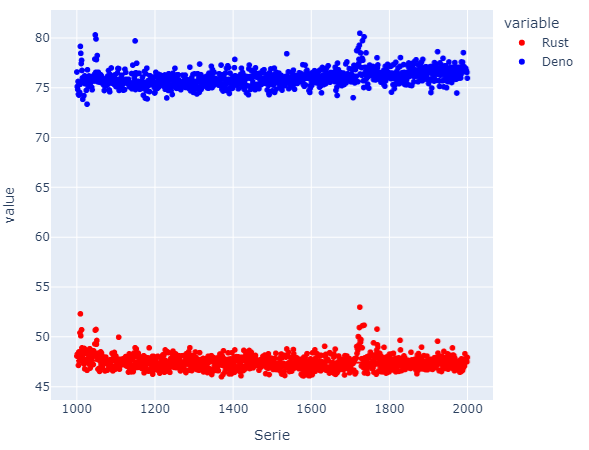
\includegraphics[width=0.52\textwidth]{hashing_lines}
    \end{figure}

    In this image, the creation of 1,000 hashes and their respective costs in milliseconds are shown, using a bcrypt cost of 14. On average, Rust is faster by 57\%.

    The trends here are not clearly defined, but two aspects are apparent from the following graphs.

    \begin{figure}[H]
        \centering
        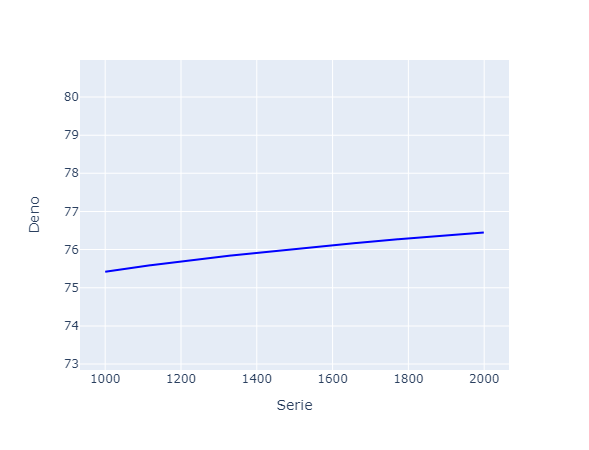
\includegraphics[width=0.52\textwidth]{trend_hash_deno}
    \end{figure}

    \begin{figure}[H]
        \centering
        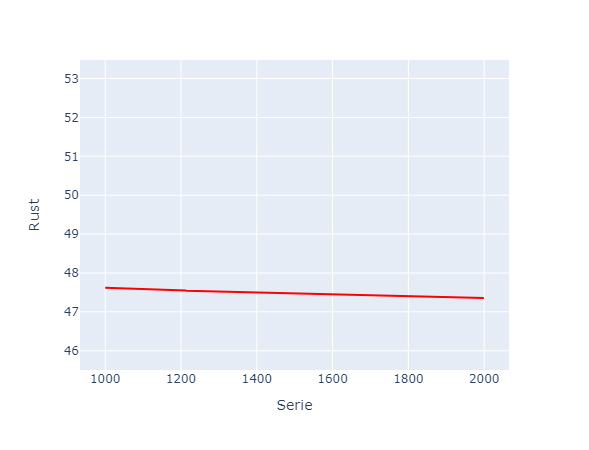
\includegraphics[width=0.52\textwidth]{images/trend_hash_rust.png}
    \end{figure}

    From the data, some observations can be made:
    \begin{itemize}
        \item The cost of hashing will increase more rapidly than it does in Rust.
        \item Rust will be more stable and experience less growth.
    \end{itemize}

    \subsubsection{Secret boxes}

    Secret boxes are a concept introduced by the library NaCl. A secret box is essentially a box with only one lock, serving as a metaphor for synchronous cryptography. The algorithm to be used in this project is a variant called \textit{tweetnacl}, which replicates the exact functionality of NaCl but fits within 100 tweets.

    The focus of this library is on speed and minimal disk footprint for both developers and users.

    \begin{figure}[H]
        \centering
        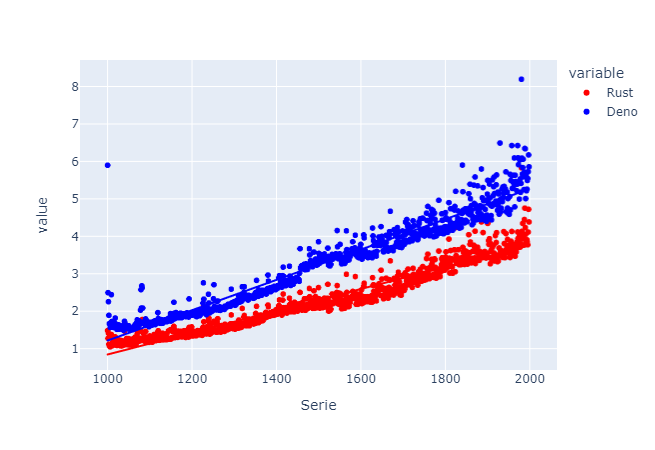
\includegraphics[width=0.52\textwidth]{images/secretbox_lines}
    \end{figure}

    In the graph, there are some Deno results that deviate from the predicted outcomes. Since these anomalies do not appear in the Rust variant, they likely arise from variations in V8's \textit{heat} function. In V8, when a function is called, it gains \textit{heat}, meaning it gets cached for later use. If a function is executed frequently, it gets stored in machine code to maximize performance.

    In this example, it can once again be observed that JavaScript is more unstable than Rust and tends to experience greater growth in computational cost.

    \begin{figure}[H]
        \centering
        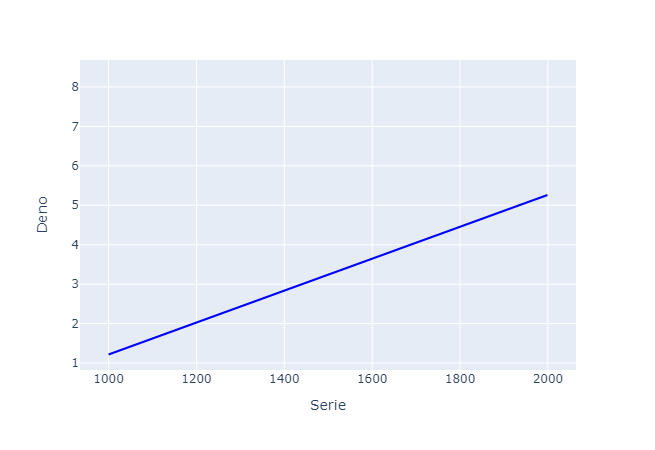
\includegraphics[width=0.52\textwidth]{trend_secretbox_deno}
    \end{figure}

    \begin{figure}[H]
        \centering
        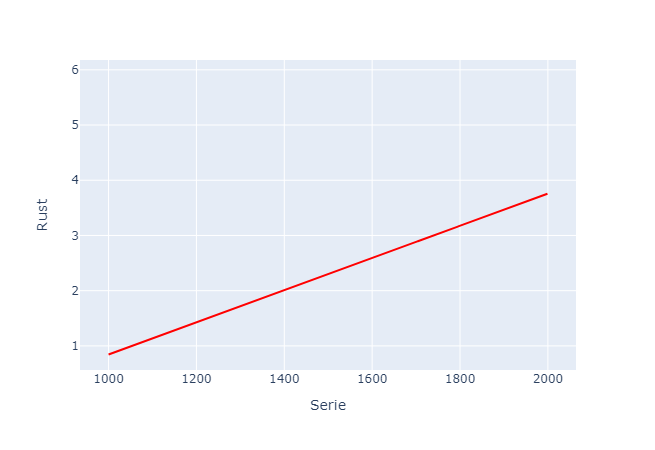
\includegraphics[width=0.52\textwidth]{images/trend_secretbox_rust}
    \end{figure}

    From the data, some observations can be made:
    \begin{itemize}
        \item The cost of encrypting will rise more rapidly in JavaScript than it does in Rust.
        \item Rust will be more stable and experience less growth.
    \end{itemize}


    \subsubsection{Box}

    A box is essentially a container with two locks, serving as another metaphor for asymmetric encryption. Like the previous algorithm, this one is based on \textit{tweetnacl}.

    \begin{figure}[H]
        \centering
        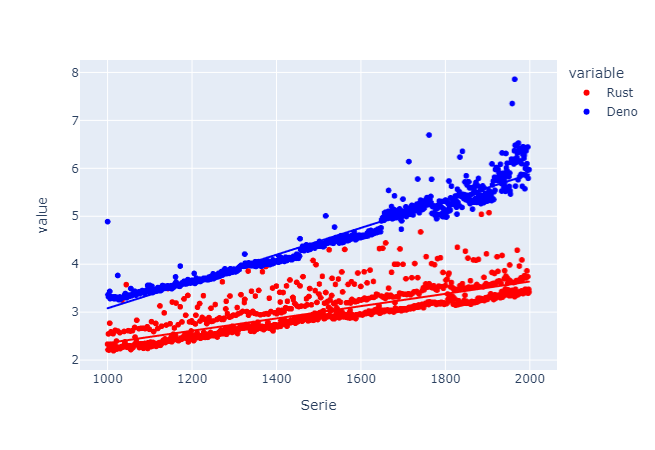
\includegraphics[width=0.52\textwidth]{images/box_lines}
    \end{figure}

    In this final algorithm, Rust outperforms Deno significantly, even though its performance is more dispersed.

    \begin{figure}[H]
        \centering
        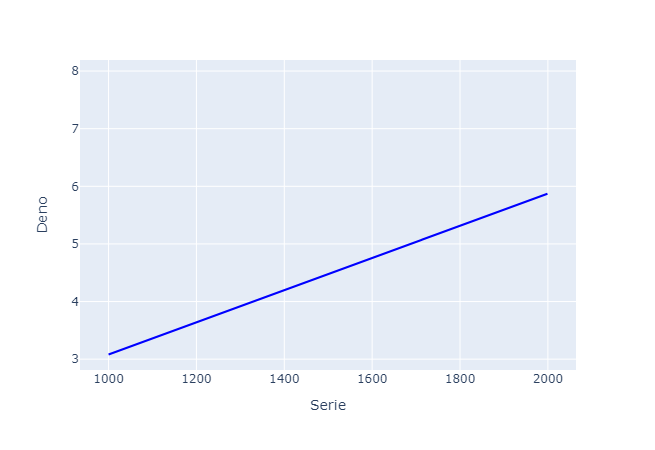
\includegraphics[width=0.52\textwidth]{trend_box_deno}
    \end{figure}

    \begin{figure}[H]
        \centering
        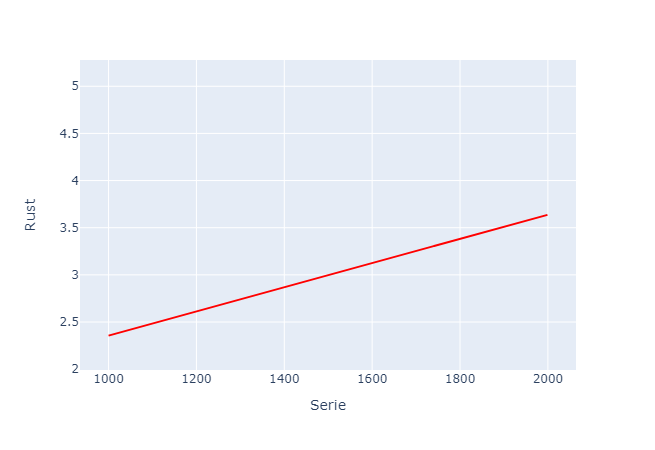
\includegraphics[width=0.52\textwidth]{images/trend_box_rust}
    \end{figure}

    From the data, some aspects can be deduced:
    \begin{itemize}
        \item The cost of encrypting will rise more rapidly in Deno than in Rust.
        \item Rust will be more stable and experience less growth.
    \end{itemize}

    \section{Conclusions}

    This project is a success both in theory and in practice. The motivation for this project was to accelerate the performance of JavaScript-based projects, which seem to be emerging every day. One such project is IPFS (InterPlanetary File System), which primarily utilizes this suite of algorithms in its operations. This suite of libraries is specifically used in \verb|OrbitDB|, a useful library for creating popular databases in a distributed manner.

    To give a brief overview, these libraries are based on distributed technologies, which involve sending small pieces of information from many users to a single user. It may be necessary to concatenate pieces of information from multiple peers to fulfill a request, making speed critical for this method of information transport.

    IPFS is rooted in a JavaScript project and experiences all the associated growing pains. Despite the IPFS team spending considerable time optimizing the library, they are still limited by the maximum capacity of JavaScript.

    IPFS came close to solving this \textit{issue} when they implemented the protocol in Go, an excellent language with a C ABI and a decent WASM implementation. However, JavaScript is still used at the core. There are multiple implementations of the IPFS protocol, but the official one is the most commonly used, significantly slowing down the network.

    Using this library will benefit performance both on the desktop and in the browser.

    Another good benefit to the future of developers is the fully virtualized environment. This can be achived by using a Docker container. This will allow the developer to have a fully virtualized environment with all the dependencies needed to run the project. This will allow the developer to have a fully reproducible environment. It also prevents any attack on the developer's machine, as the code will be running in a container.

    Microsoft is leading this space with their Visual Studio Code Remote Containers. This is a feature that allows the developer to open a folder in a container. This is a very good feature for the developer experience, as the developer does not need to install any dependencies on their machine. This is also a very good feature for security, as the developer does not need to install any dependencies on their machine.

    It has a local counterpart called \verb|dev-containers| that works exactly the same way but hosted locally.


\end{multicols}
\begin{thebibliography}{9}
    \bibitem{TFG}
    Aitor Ruiz Garcia (2022) \emph{Investigación y desarrollo del uso de la tecnoloía blockchain como validador de indentidades distribuidas y su aplicación en la Universidad de Deusto}.

    \bibitem{NPMCOUNT}
    Wikipedia (2023) \emph{npm}.

    \bibitem{BADNPM}
    Mateusz Morszczyzna (2017) \emph{What's really wrong with node\_modules and why this is your fault}.

    \bibitem{BADFAKER}
    Ax Sharma (2022) \emph{npm Libraries 'colors' and 'faker' Sabotaged in Protest by their Maintainer—What to do Now?}.

    \bibitem{VERGEFAKER}
    Emma Roth (2022) \emph{Open source developer corrupts widely-used libraries, affecting tons of projects}, The Verge.

    \bibitem{NODEGYP}
    Node (2023) \emph{node-gyp - Node.js native addon build tool}.

    \bibitem{TypeScript}
    Wikipedia (2023) \emph{TypeScript}.

    \bibitem{Polyfill}
    Mozilla (2023) \emph{MDN Web Docs Glossary: Definitions of Web-related terms - Polyfill}.

    \bibitem{DenoSec}
    Deno (2023) \emph{Deno - Permissions}.

    \bibitem{Bundler}
    Diego Salinas Gardón (2022) \emph{The Complete JavaScript Module Bundlers Guide}.

    \bibitem{WASM}
    Mozilla (2023) \emph{MDN Web Docs - WebAssembly}.

    \bibitem{Github}
    Github (2023) \emph{About GitHub-hosted runners}.

    \bibitem{Bcrypt}
    Wikipedia (2023) \emph{Bcrypt}.

    \bibitem{IPFS}
    IPFS team (2022) \emph{Design and Evaluation of IPFS: A Storage Layer for the Decentralized Web}.

    \bibitem{WASMBAD}
    \textit{juj} (2021) \emph{Wasm needs a better memory management story}

\end{thebibliography}
\end{document}